% 互余角关系图：同一直角三角形 A、B 互余，α 的对边 = β 的邻边
\documentclass[tikz,border=4pt]{standalone}
\usepackage{ctex}
\usepackage{amsmath}
\begin{document}
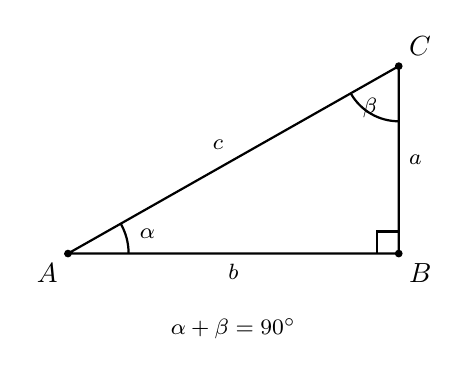
\begin{tikzpicture}[scale=1.4, thick]
  \coordinate (A) at (0,0);
  \coordinate (B) at (3,0);
  \coordinate (C) at (3,1.7);
  \draw (A) -- (B) -- (C) -- cycle;
  \draw (2.8,0) -- (2.8,0.2) -- (3,0.2);
  % α at A
  \draw (0.55,0) arc (0:30:0.55);
  \node at (0.72, 0.18) {\footnotesize $\alpha$};
  % β at C
  \draw (3,1.2) arc (-90:-150:0.5);
  \node at (2.74, 1.32) {\footnotesize $\beta$};

  \fill (A) circle (1pt); \fill (B) circle (1pt); \fill (C) circle (1pt);
  \node[below left] at (A) {$A$};
  \node[below right] at (B) {$B$};
  \node[above right] at (C) {$C$};
  \node[below] at (1.5,0) {\footnotesize $b$};
  \node[right] at (3, 0.85) {\footnotesize $a$};
  \node[above left] at (1.5, 0.85) {\footnotesize $c$};
  \node[below] at (1.5,-0.5) {\footnotesize $\alpha+\beta=90^\circ$};
\end{tikzpicture}
\end{document}
